%ब
\section{Cassandra} \label{s:Cassandra}

Cassandra is a distributed data storage system initially developed by Facebook
 for satisfying the needs of large web applications, where
scalability and response time to user requests are critical(\todo{cite BOOK}).
It's development is now undertaken by Apache (Gunda, 2010) and is being used by
many large web applications and large organisations like Facebook, Twitter,
Cisco, Digg, Reddit etc (\todo{cite BOOK}).

Cassandra is based on the column-oriented key value data model and stores data
in tables that have columns, super column family rows, row keys etc.
These have been explained in Section~\ref{s:key-value-data-model}

Cassandra is run as a single Java process run on a machine and is specifically
designed to work efficiently across different machines and across multiple data
centers, even data centers that are geographically distributed. The details of
the distributed nature is abstracted from  the user and the it appears to the
user that everything is stored on a single machine. This distributed nature
makes Cassandra better utilised when it is run on multiple machines in a cluster
(\todo{Perham, 2010a, BOOK}).

A cluster can be considered as the outermost structure in the data model of
Cassandra. All the machines operating together on which a Cassandra database
relies for holding its data  forms a cluster or ring of nodes
(Figure~\ref{f:cluster}).In such a cluster, all the machines or nodes are
connected to each other and each node is aware of all their peers in the
cluster.

\begin{figure}[h] \centering
	% 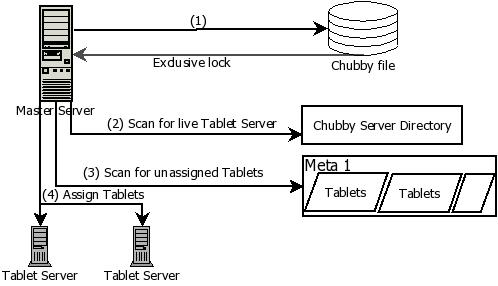
\includegraphics[width=5cm,   height=5cm]{. /figure/random. jpg}
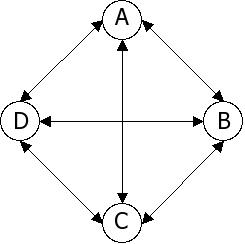
\includegraphics[width=.3\textwidth]{./figure/Cassandra/Cassandra-cluster.png}
	\caption{A cluster of nodes in Cassandra}\label{f:cluster}
\end{figure}

Distributed system are prone to conflicts as many users could be issuing
requests on data items from any of the nodes. Any distributed system should
carefully consider conflict resolution and adopt design approaches which would
resolve such conflicts efficiently. Conflicts arise either at read or write
operations.
The design approach should either make the system resolve such conflicts either
during one of these operations, deciding the system be either readable at all
times or writable. Cassandra optimises its performance by adopting the design
approach of resolving conflicts during read operations, making Cassandra always
writable.

All nodes in a Cassandra cluster applies the same architectural features
fundamental to Cassandra like bootstrapping, load balancing, replicating and
partitioning data, failure detection mechanisms etc. Some of the key
architectural concepts are explained in the following sub-section.



\subsection{Architecture} \label{ss:Cassandra-architecture}

Cassandra adopts a lot of its architectural concepts from other popular
distributed key-value data storage systems on the cloud, like Google's Bigtable
and Amazon's Dynamo. Overtime these adopted concepts evolved and developed new
features , some of which became specific to Cassandra's architecture. These
architectural concepts gave Cassandra its popular features like elastic
scalability, fault tolerance, high availability and high performance Cassandra's
architecture involves many sophisticated and complex theoretical as well as
mathematical concepts, some of which are discussed below. Discussing every
concept is beyond the scope of this research.

% The nodes in a cluster communicate with each other using the P2P communication
% protocol, Gossip. This protocol involves many complex mathematical models and
% help in significantly reducing the time taken to propagate requests from node
% to node (Raja, 2010).This protocol broadcasts any membership changes to all
% the nodes and allows nodes to reconcile such changes with its peer nodes.
% Using Gossip, nodes thus update their routing information about other nodes
% periodically. This also allows nodes to perform load balancing operations,
% i.e., some workload is given to other nodes, when a node fails or has a high
% workload.



\begin{description}
\item[Peer-Peer Distribution Model:] Within a Cassandra cluster, all the nodes
are considered equal or identical in sharing responsibilities and
performing operations, in other words, all nodes are configured as peers and no
single node is a master or slave.  This is unlike traditional\acp{DBMS} that
are distributed, where nodes are configured such that they have different
responsibilities and roles. For example, some or one of the nodes is a master
and others are slaves.
Such a centralised configuration improves reading data, as data can be read from
any of the slave nodes, but write requests are always sent to the master node.
This model thus puts a lot of additional load on the master and also is prone to
failure if the single master node is offline.

The peer-peer model in Cassandra is decentralized and  provides high data
availability since failure of some of the nodes does not affect the service of
the cluster, as other nodes can carry out the same operation or role. Similarly
this model makes new node additions to the cluster easy. Since nodes are
similar, no specific role has to be assigned to the new nodes, they just have to
be added to the cluster. Addition of nodes invokes the bootstrapping process,
which is explained later.

In a Cassandra cluster nodes use the peer-peer communication protocol called
Gossip for relaying information within the ring. Nodes sent state information at
regular time intervals using the gossiper so that other nodes in the ring can
know their status.

This is essential for failure detection in Cassandra. A gossip session is
initiated with a random node within the cluster during regular intervals where
the initiator node  sends a \texttt{sync} message to another node. If  the
recipient node is active it would return an \texttt{ack} message to the gossiper
or the initiator. The initiator then sends a second \texttt{ack} message to
acknowledge the transmission and the gossip session is completed. If the
recipient node does not send an \texttt{ack} message it is marked as dead and
this information is logged.

When a node is found to be offline, after a gossip session, Cassandra implements
the \textit{hinted handoff} feature, to ensure that the operations that were
sent to the failed node are not lost (Figure~\ref{f:hinted handoff}). If a write
request was sent to the failed node, the node that now receives it would create
a small hint message with the information about the write request. This
recipient node would use gossip sessions to check the status of the failed node
so that it can give the hint to the failed node once it is alive again. A hinted
handoff acknowledgement is
considered a successful write operation if the consistency level set by the
user, discussed under Eventual Consistency, is low., otherwise it is not
considered as successful and these hinted writes will not be readable. The
hinted handoff feature can be disabled in Cassandra if needed, depending on the
suitability of the application using Cassandra.
\begin{figure}[h] 
	\centering
	%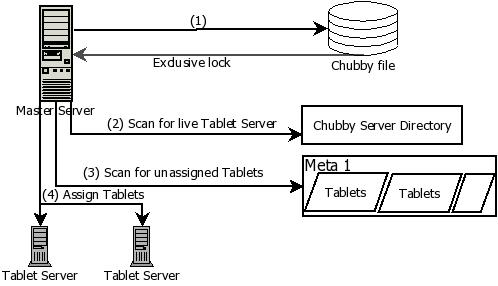
\includegraphics[width=5cm,   height=5cm]{. /figure/random. jpg}
	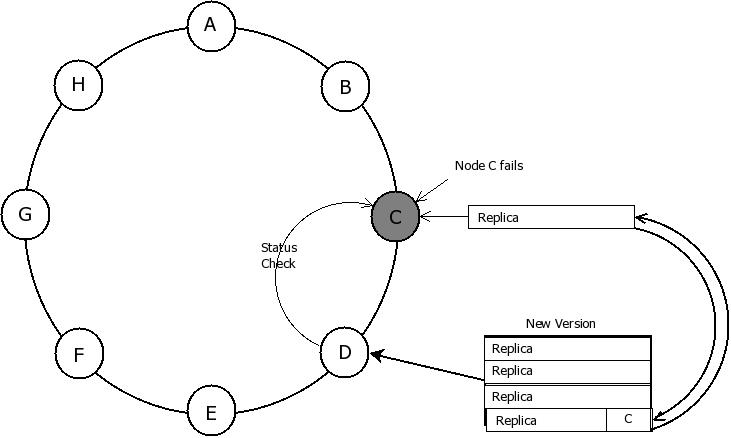
\includegraphics[width=.6\textwidth]{./figure/Cassandra/Hinted-handoff.png}
	\caption{Hinted handoff in Cassandra}\label{f:hinted handoff}
\end{figure}

\item[Bootstrapping:] When a node starts for the first time, it checks its
configuration files to retrieve the location information of some of the
initial contact nodes or seed nodes.  It then chooses a random token, which is a
random value, for its position in the cluster and this token information of the
new node is gossiped to the other nodes in the cluster. This enables nodes to
have the routing information of all the peers in a cluster to send requests.
This is illustrated in Figure~\ref{f:bootstrap}, where \texttt{H} is a new node
joining the cluster after checking its configuration files and getting a token to join
the cluster. Its state information is then gossiped through the cluster. Node
\texttt{F} splits its ranges and send it to \texttt{H}, making \texttt{H}
responsible for the keys of that range.

\newpage

\begin{figure}[H]
	\centering
	%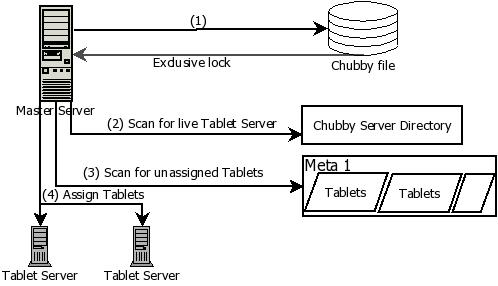
\includegraphics[width=5cm,   height=5cm]{. /figure/random. jpg}
	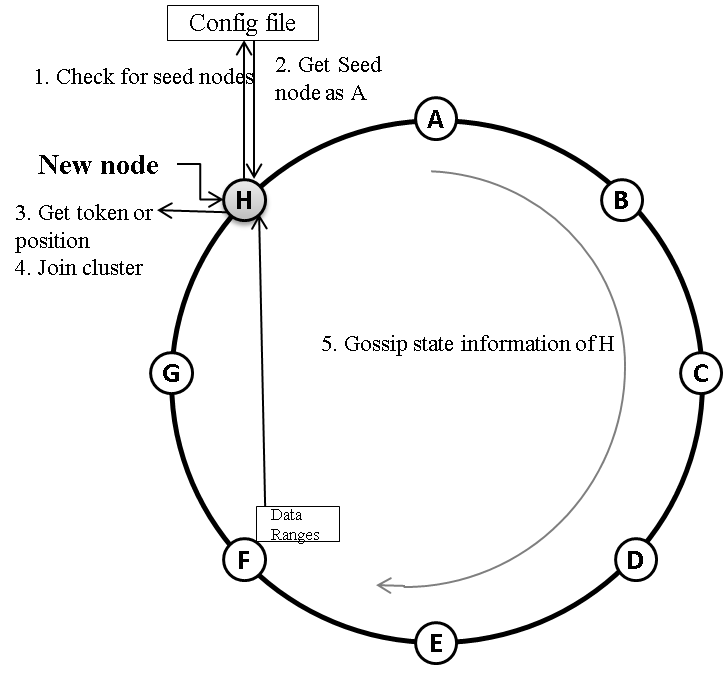
\includegraphics[width=.6\textwidth]{./figure/Cassandra/Bootstrapping.png}
	\caption{Bootstrapping in Cassandra}\label{f:bootstrap}
\end{figure}

The token assigned to a new node would help balance the load of an overloaded
node, as some of the operations are transferred to the new node after all nodes
in the cluster know of its existence.  The new node thus is assigned a range
which belonged to another node. The bootstrapping algorithm renders Cassandra
the architectural feature of elastic scalability where adding new nodes is
simple and does not affect other nodes or operations in the cluster. This also
helps in load balancing and ensuring that the cluster has no bottlenecks of
overloaded nodes clogging the cluster. To achieve elastic scalability data has
to be dynamically partitioned between the nodes, which is explained next.

\item[Partitioning Data:] For  elastic scalability and efficient load balancing
Cassandra adopts the consistent hashing used by Amazon's Dynamo to partition
data over the nodes.(\todo{DeCandia et al.(2007)}). In consistent hashing, after
a node is assigned a place in a cluster, data objects that are identifiable by
their keys, are assigned to the node. The key of each data object is hashed and
the data object is sent to the node that is larger than this hashed value
(Figure~\ref{f:consistent hashing}). 
This node is called the coordinator node
for those keys stored on it.

\begin{figure}[h]
	\centering
	%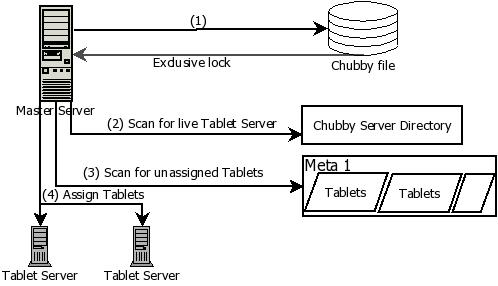
\includegraphics[width=5cm,   height=5cm]{. /figure/random. jpg}
	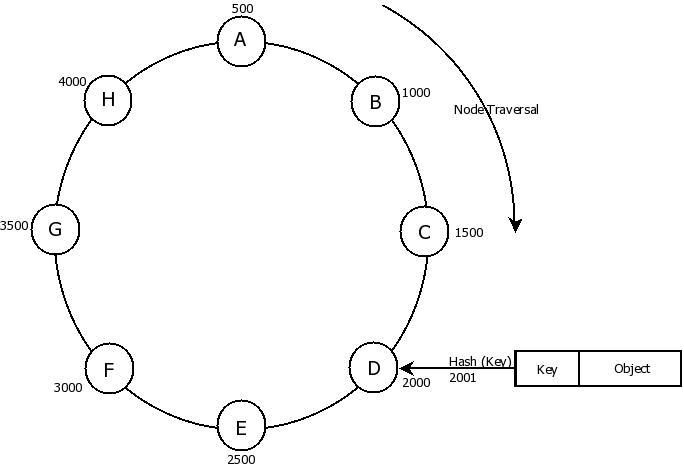
\includegraphics[width=.6\textwidth]{./figure/Cassandra/Consistent-hashing-Cassandra.png}
	\caption{Consistent hashing in Cassandra}\label{f:consistent hashing}
\end{figure}

Partitioning data helps in load balancing as well as scalability of a cluster to
distribute workload to new nodes without affecting the performance of the
entire cluster. Additionally, in Cassandra better performing nodes are assigned
multiple points in the ring, making them virtual nodes and these nodes are assigned
  workloads from failed nodes or overloaded nodes. 

  \item  [Replication strategy]: For data to be always available to
  the users at all times, irrespective of failures, Cassandra uses a
  replication strategy. This involves replicating every object
  across several nodes by replicating a data item to N number of hosts, where N
  is the number of replicas that the user specifies. After consistent
  hashing, data items are assigned their coordinator nodes and these  nodes
  replicate the assigned objects (DeCandia et al., 2007). After saving the data
  items on locally, the coordinator nodes replicates the data items to N-1
  hosts. A preference list contains routing information about all the
  coordinator nodes that are responsible for storing a key (Figure~\ref{f:
  preference-list})which makes every node in the ring aware of which nodes are
  responsible for a key.
 
\begin{figure}[h]
	\centering
	%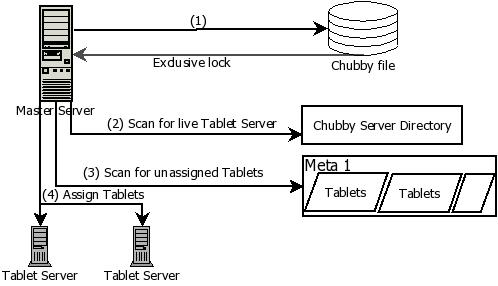
\includegraphics[width=5cm,   height=5cm]{. /figure/random. jpg}
	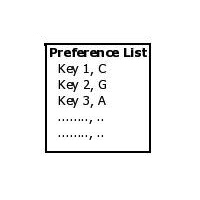
\includegraphics[width=.4\textwidth]{./figure/Cassandra/Preference-list.png}
	\caption{A preference list example}\label{f: preference-list}
\end{figure}

Such a replication strategy makes Cassandra highly available as data items are
available from any node in the cluster and node failures do not
affect  data availability. All the nodes would know what ranges of key a
peer node is responsible for from the preference list and this helps in routing
requests to the correct nodes. 

Users can set the level of replication they would prefer, by setting the
replication factor to the number of nodes the users would like to use for
replication. In other words, replication factor tells the cluster how many
copies to save of a single data item. Setting the replication factor to a large
number would help in higher consistency of data items, but replicating data
items to a large number of nodes, each time there is an operation on it,  can
adversely affect the performance.

  \item [Eventual Consistency]:Consistency refers to the ideal scenario where
  all users read the same value of a data item, even when concurrent update
  operations are done on the data item.As mentioned previously, Cassandra opts
  for '\texttt{A}' and '\texttt{P}' of the CAP theorem and allows users to
  determine the level of consistency they would prefer by letting the users set
  the consistency level, which would tell the cluster how many
  replicas should acknowledge operations done on them, for the replicas to be
  considered consistent and up to date. Low consistency levels are considered
  better for performance as higher consistency levels involve more time
  since nodes have to wait to receive acknowledgements from more replicas.
  Letting the users decide the consistency level and replication factor means
  the amount of consistency is ascertained by the users. 

  To ensure the consistency between the nodes that the user sets in the
  consistency level, Cassandra uses the eventual consistency model, which is
  different from the commonly used strict consistency model in traditional
  \acp{DBMS} .
  Strict consistency models ensure that a read operation always returns the most
  update values. This is practical only in situations where the system using
  such a model is dependant on a single machine, where the operations are
  performed sequentially. But in distributed systems, where more machines are
  used, this leads to various conflicts when more than one user is involved. For
  distributed systems a weaker form of consistency, called eventual consistency
  is considered better (\todo{cite BOOK and marked papers}).
  
   Eventual consistency is where every replica agrees to the most recent value
   after a certain point in time and allows updates to be propagated to all the
   replicas asynchronously (Figure~\ref{f: eventual consistency}) (Henry, 2008).
   Thus, all replicas would be consistent eventually after a certain period of
   time, generally a small number of milliseconds \todo{cite book}.
   This requires that the replicas update the values in an order. Eventual
   consistency is useful when a distributed system has to scale greatly.
   If $N$ is the number of nodes containing replicas or the
  replication factor, $W$ is the number of replicas that should acknowledge a
  write operation and $R$ is the number of replicas that have to be contacted
  for a read operation (or the consistency level),
  then eventual consistency can be summarized as:%\\*
  
  \begin{equation}
  	W + R <= N \nonumber  
  \end{equation}
  
  This means that the consistency is not strict as the number of nodes to be
  contacted for a write or read operation is lesser than the number of nodes
  that hold the replicas.
  
  Cassandra performs \textit{read repairs} to make replicas of data consistent
  with the latest versions. Data inconsistencies are determined after checking
  the timestamps of the replicas by the node.  When during a read operation a
  node finds out that the replicas it received from a node  was not consistent with
  replicas on newer nodes, a read repair is performed on the node with the
  outdated replicas. This means that the older
  nodes are sent a write operation with the latest data. 
  
  \begin{figure}[H]
\centering
	% 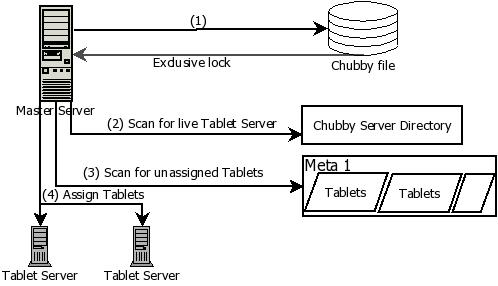
\includegraphics[width=5cm,   height=5cm]{. /figure/random. jpg}
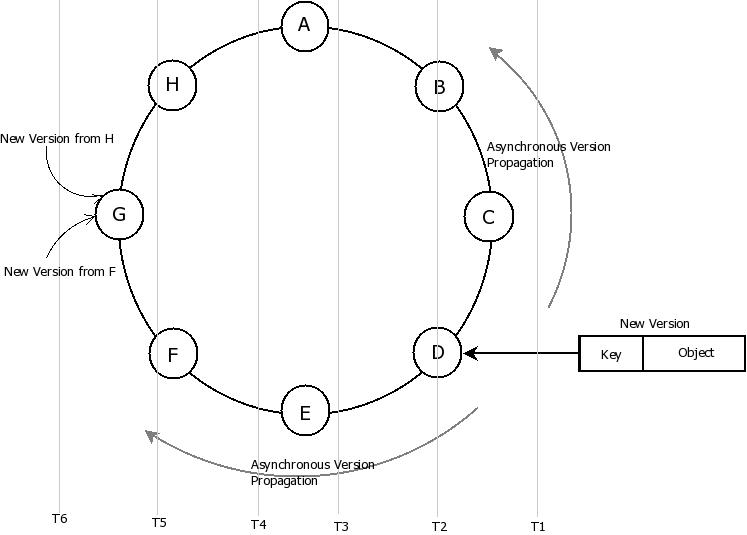
\includegraphics[width=.7\textwidth]{./figure/Cassandra/Eventual-consistency-Cassandra.png}
	\caption{Eventual Consistency in Cassandra}\label{f: eventual consistency}
\end{figure}
   This time delay in updating all replicas could translate to latency in a
   large cluster of
  Cassandra nodes, where consistency level and replication factor is high. 
  
% 	  \begin{center}
% 	  \textbf{\texttt{\emph{W} + \emph{R}} \textless = \texttt{\emph{N}}}
% 	  \end{center}
  
  In Cassandra, users have two options while deciding the consistency level:
  single read and the quorum read. In a single read, the first data or replica
  that a node receives from another node is returned as a response to user's
  read request (Figure~\ref{f:singleread}). In a  quorum read, the node that
  receives a read request collects   replicas of data from majority of the available nodes in
  the cluster and returns the most updated data to the user (Figure~\ref{f:quorumread}).
  Quorum reads are slower when compared to single reads, but these prevent stale
  data to be returned.
  
    
  		 \begin{figure}[H]
			\centering
			% 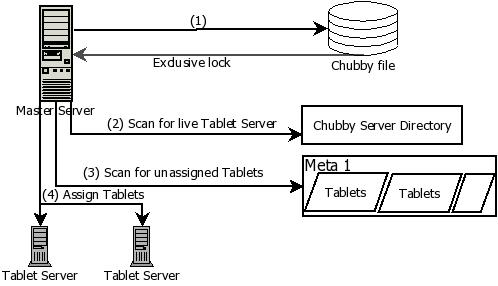
\includegraphics[width=5cm,   height=5cm]{. /figure/random. jpg}
			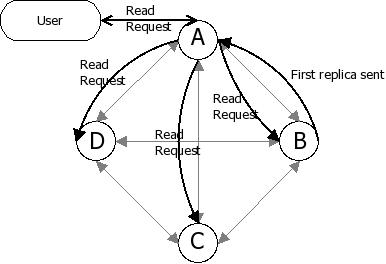
\includegraphics[width=.5\textwidth]{./figure/Cassandra/Single-Read-Cassandra.png}
		
			\caption{Single Read in Cassandra}\label{f:singleread}
		\end{figure}
 
		 \begin{figure}[H]
			\centering
			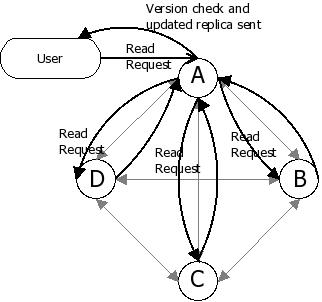
\includegraphics[width=.4\textwidth]{./figure/Cassandra/Quorum-read-Cassandra.png}
		
			\caption{Quorum Read in Cassandra}\label{f:quorumread}
		\end{figure}


  
  \item [\ac{SEDA}:] \ac{SEDA} is a concurrency model designed for concurrent
  Internet services, which allows a single operation starting within a single
  thread to let the thread pass the operations to other threads. The work is
  divided into stages, where a stage comprises of an incoming queue, event
  handler and an associated thread pool. This thread pool decides which stages
  to be executed. This is unlike conventional applications where operations are
  run in a single thread. Such a concurrency model helps Cassandra enjoy great
  increase in performance as a stage can be
  controlled by different thread pools that also help in managing the available
  resources like disk space, network bandwidth for the stage to complete the
  work. Work that is divided into stages are mostly the operations like read,
  gossip, load balancing and the like.
  
\end{description}
\subsection{ Write and Read operations}
When users wish to write data into Cassandra tables, they send a write request
to a random node in the cluster (Figure~\ref{f:writeRead}). This node acts as the proxy
and writes the data to the whole cluster, thus efficiently replicating the data.
A user can set the number of nodes that should have the
replicated data copied on it and these replicas are saved on to nodes in the
same data centre and on other nodes in the other data centres. These nodes would act
as proxies when they receive requests from users (Perham, 2010a). This way even
if nodes fail, data is recoverable from other nodes.
		

Similarly, when a user makes a read request to a node, the node acts as a proxy
node and forwards the request to all the other nodes in the cluster
(Figure~\ref{f:singleread}).
As mentioned before, the level of consistency is specified by the user, i.e.,
single or quorum read. Nodes return data to the user after checking the versions
of the replicas and send the latest replica to the user and perform read repairs
on other nodes in the cluster (Perham, 2010b).
The technical details of how to read and write into Cassandra is discussed in
the following chapter.

\begin{figure}[H]
			\centering
			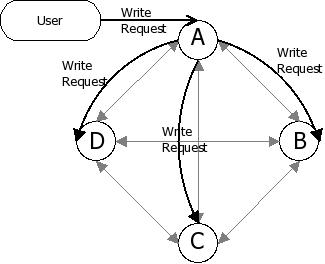
\includegraphics[width=.45\textwidth]{./figure/Cassandra/Write-Request-Cassandra.png}
						\caption{A write and read operation in Cassandra}\label{f:writeRead}
		\end{figure}
